%!TEX ROOT=formularioMatematica.tex

\section{Affinità}\label{sec:aff}
Si definisce un'affinità come una corrispondenza biunivoca tra due piani e tra punti dello stesso 
piano che trasformi rette in rette conservando il parallelismo.\\
Un'affinità generica denominata $T$ può essere espressa nei seguenti modi
\begin{equation*}
T:\,\begin{cases}
x'=ax+by+e\\
y'=cx+dy+f
\end{cases}
\end{equation*}
\begin{equation*}
T:\,\begin{bmatrix}[1]
x'\\y'
\end{bmatrix}=
\begin{bmatrix}[1]
a&b\\
c&d
\end{bmatrix}
\begin{bmatrix}[1]
x\\y
\end{bmatrix}
+\begin{bmatrix}[1]
e\\f
\end{bmatrix}
\end{equation*}
\begin{equation*}
T:\,(x,y)\mapsto(ax+by+e,cx+dy+f)
\end{equation*}
Tutte le affinità hanno il determinante della matrice dei coefficienti è sempre diverso da zero
\begin{equation*}
\begin{vmatrix}[1]
a&b\\
c&d
\end{vmatrix} = ad-cb \neq0
\end{equation*}
Se il determinante è pari a $1$ è un'isometria e quindi mantiene le distanze.\\\\

Si definisce punto unito qualunque punto che si trasforma in sé stesso, ovvero
\begin{equation*}
T(U) \equiv U (\equiv U')
\end{equation*}

Essendo le affinità proprietà binuivoche, esiste anche la trasformazione inversa, generalmente 
indicata con $T^{-1}$.\\
Per gli esercizi si vada a pagina~\pageref{ex:aff}.

\subsection{Prodotto di trasformazioni}
Se si hanno due trasformazioni $T$ e $T'$, il loro prodotto è descritto come $T\ast T'$ e si ottiene
effettuando prima $T'$ e successivamente $T$. Quindi è equivalente a $T(T'(P))$.\\
La matrice dei coefficienti si ottiene moltiplicando le due matrici $A\ast A'$.

\subsection{Traslazione}
\begin{center}
	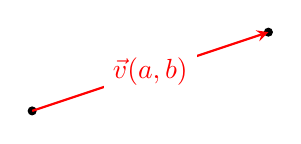
\begin{tikzpicture}
		\coordinate (A) at (1,2);
		\coordinate (B) at (4,3);
		
		\tkzInit[xmin=-1,ymin=-1,xmax=5,ymax=5]
		\tkzGrid
		\tkzAxeXY
		
		\filldraw (A) circle (0.05);
		\filldraw (B) circle (0.05);
		\draw[red, thick, -stealth] (A) -- (B)
			node[pos=0.5, fill=white, text=red]{$\vec{v}(a,b)$};
	\end{tikzpicture}
\end{center}
\begin{equation*}
\tau_{\begin{bmatrix}[0.7]
	\mathcolor{red}{a}\\\mathcolor{red}{b}
	\end{bmatrix}}:
\begin{cases}
x'= x+\mathcolor{red}{a}\\
y'= y+\mathcolor{red}{b}
\end{cases}
\end{equation*}
\begin{equation*}
\tau_{\begin{bmatrix}[0.7]
	\mathcolor{red}{a}\\\mathcolor{red}{b}
	\end{bmatrix}}^{-1}:
\begin{cases}
x = x'-\mathcolor{red}{a}\\
y = y'-\mathcolor{red}{b}
\end{cases}
\end{equation*}

\subsection{Rotazione}
\begin{center}
	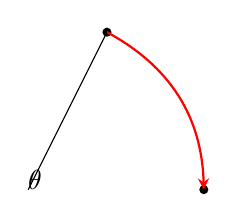
\begin{tikzpicture}
		\coordinate (A) at (1,2);
		\coordinate (B) at (2.23,0);
		\coordinate (O) at (0,0);
		
		\tkzInit[xmin=-1,ymin=-1,xmax=5,ymax=5]
		\tkzGrid
		\tkzAxeXY
		
		\filldraw (A) circle (0.05);
		\filldraw (B) circle (0.05);
		\path[thick, red, -stealth, bend left] (A) edge (B);
		\draw (O) -- (A);
		\markangle{O}{A}{B}{0.5}{1.5}{$\theta$}
	\end{tikzpicture}
\end{center}
\begin{equation*}
\rho_{O,\theta}:\,\begin{cases}
x'=x\cos\theta-y\sin\theta\\
y'=x\sin\theta+y\cos\theta
\end{cases}
\end{equation*}
\begin{equation*}
\rho_{O,\theta}:\,\begin{cases}
x=x'\cos\theta+y'\sin\theta\\
y=-y'\sin\theta+y\cos\theta
\end{cases}
\end{equation*}

\subsection{Simmetria centrale}
\begin{center}
	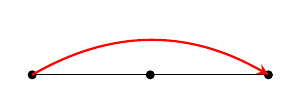
\begin{tikzpicture}
		\coordinate (A) at (-1,0);
		\coordinate (B) at (2,0);
		\coordinate (C) at (0.5,0);
		
		\tkzInit[xmin=-1.5,ymin=-1,xmax=2.5,ymax=1]
		\tkzGrid
		\tkzAxeXY
		
		\filldraw (A) circle (0.05);
		\filldraw (B) circle (0.05);
		\filldraw (C) circle (0.05);
		\draw (A) -- (B);
		\path[thick, red, bend left, -stealth] (A) edge (B);
	\end{tikzpicture}
\end{center}

\begin{equation*}
\sigma_{C(x_C,y_C)}:\,\begin{cases}
x'= -x+2x_C\\
y'= -y+2y_C
\end{cases}
\end{equation*}
\begin{equation*}
\sigma_{C(x_C,y_C)}^{-1}:\,\begin{cases}
x = -x'+2x_C\\
y = -y'+2y_C
\end{cases}
\end{equation*}

\subsection{Simmetria assiale}
\begin{center}
	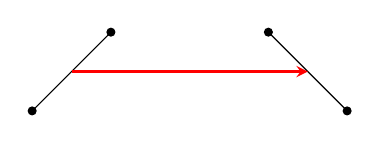
\begin{tikzpicture}
		\coordinate (A) at (-2,0);
		\coordinate (B) at (-1,1);
		\coordinate (C) at (1,1);
		\coordinate (D) at (2,0);
		
		\tkzInit[xmin=-3,ymin=-1,xmax=3,ymax=2]
		\tkzGrid
		\tkzAxeXY
		
		\filldraw (A) circle (0.05);
		\filldraw (B) circle (0.05);
		\filldraw (C) circle (0.05);
		\filldraw (D) circle (0.05);
		\draw (A) -- (B);
		\draw (C) -- (D);
		\draw[-stealth, red, thick] (-1.5,0.5) -- (1.5,.5);
	\end{tikzpicture}
\end{center}

\subsubsection{Rispetto a $r:\,y=y_0$}
\begin{equation*}
\sigma_r:\,\begin{cases}
x'= x\\
y'= -y+2y_0
\end{cases}
\end{equation*}

\subsubsection{Rispetto a $r:\,x=x_0$}
\begin{equation*}
\sigma_r:\,\begin{cases}
x'= -x+2x_0\\
y'=y
\end{cases}
\end{equation*}

\subsubsection{Rispetto a $r:\,y=mx+q$}
\begin{equation*}
\sigma_r:\,\begin{cases}
x'=\frac{1}{1+m^2}[(1-m^2)x+2my-2mq]\\
y'=\frac{1}{1+m^2}[2mx+(m^2-1)y+2q]
\end{cases}
\end{equation*}

\begin{equation*}
\sigma_r^{-1}:\,\begin{dcases}
x=\frac{1}{1+m^2}[(1-m^2)x +2my'-2mq]\\
y=\frac{1}{1+m^2}[2mx'+(m^2-1)y'+2q]
\end{dcases}
\end{equation*}

\subsection{Similitudine}
\begin{center}
	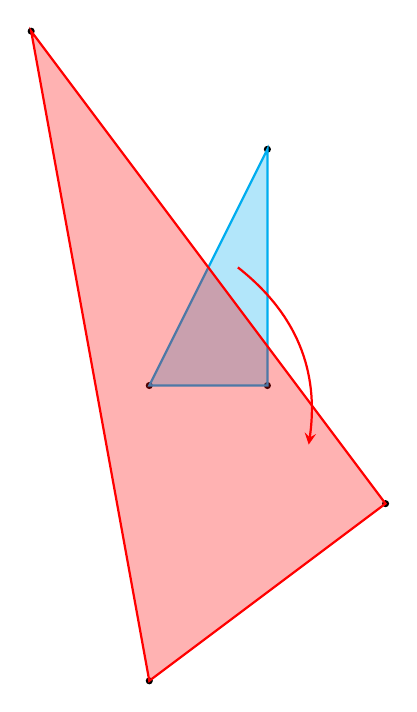
\begin{tikzpicture}[scale=0.75]
		\coordinate (A) at (-2,0);
		\coordinate (B) at (0,4);
		\coordinate (O) at (0,0);
		\coordinate (C) at (-4,6);
		\coordinate (D) at (-2,-5);
		\coordinate (E) at (2,-2);
		
		\tkzInit[xmin=-5,ymin=-6,xmax=3,ymax=7]
		\tkzGrid
		\tkzAxeXY
		
		\filldraw (A) circle (0.05);
		\filldraw (B) circle (0.05);
		\filldraw (C) circle (0.05);
		\filldraw (D) circle (0.05);
		\filldraw (E) circle (0.05);
		\filldraw (O) circle (0.05);
		
		\filldraw[thick, cyan, fill opacity = 0.3] (A) -- (B) -- (O) -- cycle;
		\filldraw[thick, red, fill opacity = 0.3] (C) -- (D) -- (E) -- cycle;
		\path[-stealth, red, thick, bend left] (-0.5,2) edge (0.7,-1);
	\end{tikzpicture}
\end{center}

\begin{equation*}
\Sigma:\,
\begin{cases}
\begin{cases}
x'= ax-by+e\\
y'= bx+ay+f
\end{cases}\text{Se diretta, }\det A = \begin{vmatrix}[1]
a&-b\\b&-a
\end{vmatrix}>0\\
\begin{cases}
x'=ax+by+e\\
y'=bx-ay+f
\end{cases}\text{Se indiretta, }\det A = \begin{vmatrix}[1]
a&b\\b&-a
\end{vmatrix}<0
\end{cases}
\end{equation*}
Il rapporto di similitudine è pari a 
\begin{equation*}
k = \sqrt{a^2+b^2}
\end{equation*}

\subsection{Omotetia}
\begin{center}
	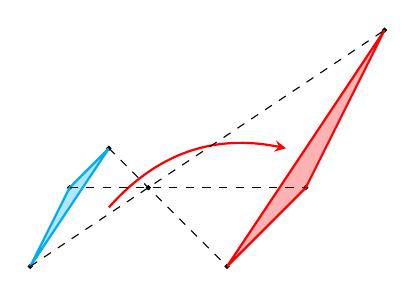
\begin{tikzpicture}[scale=0.5]
		\coordinate (A) at (-2,0);
		\coordinate (B) at (-1,1);
		\coordinate (O) at (0,0);
		\coordinate (C) at (-3,-2);
		\coordinate (D) at (4,0);
		\coordinate (E) at (2,-2);
		\coordinate (F) at (6,4);
		
		\tkzInit[xmin=-4,ymin=-3,xmax=7,ymax=5]
		\tkzGrid
		\tkzAxeXY
		
		\filldraw (A) circle (0.05);
		\filldraw (B) circle (0.05);
		\filldraw (C) circle (0.05);
		\filldraw (D) circle (0.05);
		\filldraw (E) circle (0.05);
		\filldraw (F) circle (0.05);
		\filldraw (O) circle (0.05);
		
		\filldraw[thick, cyan, fill opacity = 0.3] (A) -- (B) -- (C) -- cycle;
		\filldraw[thick, red, fill opacity = 0.3] (D) -- (E) -- (F) -- cycle;
		\path[-stealth, red, thick, bend left] (-1,-0.5) edge (3.5,1);
		\draw[dashed] (A) -- (D);
		\draw[dashed] (B) -- (E);
		\draw[dashed] (C) -- (F);
	\end{tikzpicture}
\end{center}

\begin{equation*}
\omega_{C,a}:\,\begin{cases}
x'=a(x-x_C)+x_C\\
y'=a(y-y_C)+y_C
\end{cases} \rightarrow
\begin{cases}
x'= ax+h\\
y'= ay+k
\end{cases}
\end{equation*}

\subsection{Dilatazione}
\begin{center}
	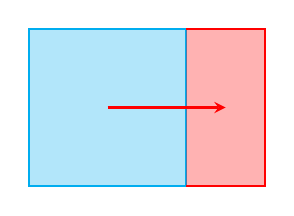
\begin{tikzpicture}
		\tkzInit[xmin=-1,ymin=-1,xmax=4,ymax=3]
		\tkzGrid
		\tkzAxeXY
		\filldraw[thick, cyan, fill opacity = 0.3] (0,0) -- (2,0) -- (2,2) -- (0,2) -- cycle;
		\filldraw[thick, red, fill opacity = 0.3] (2,2) -- (3,2) -- (3,0) -- (2,0);
		\path[-stealth, thick, red] (1,1) edge (2.5,1);
	\end{tikzpicture}
\end{center}

\begin{equation*}
\delta_{x,k}:\,\begin{cases}
x'=kx\\
y'=y
\end{cases}\quad\delta_{y,k}:\,\begin{cases}
x'=x\\
y'=ky
\end{cases}
\end{equation*}

\subsection{Inclinazione}
\begin{center}
	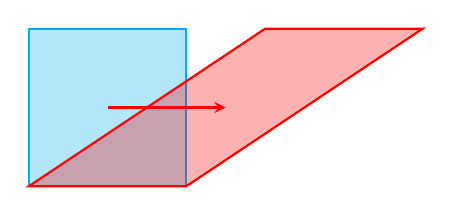
\begin{tikzpicture}
		\tkzInit[xmin=-1,ymin=-1,xmax=6,ymax=3]
		\tkzGrid
		\tkzAxeXY
		\filldraw[thick, cyan, fill opacity = 0.3] (0,0) -- (2,0) -- (2,2) -- (0,2) -- cycle;
		\filldraw[thick, red, fill opacity = 0.3] (0,0) -- (2,0) -- (5,2) -- (3,2) -- cycle;
		\path[-stealth, thick, red] (1,1) edge (2.5,1);
	\end{tikzpicture}
\end{center}
\begin{equation*}
\xi_{x,k}:\,\begin{cases}
x'=x_ky\\
y'=y
\end{cases}\quad\xi_{y,k}:\,\begin{cases}
x'=x\\
y'=y+kx
\end{cases}
\end{equation*}
